\documentclass{article}
\usepackage[french]{babel}
\usepackage[T1]{fontenc}
\usepackage[autolanguage,np]{numprint} % tableau spécial
\usepackage[left=2cm,right=2cm,top=2cm,bottom=2cm]{geometry}
\usepackage{fancyhdr}
\pagestyle{fancy}
\chead{Titre du document}
\usepackage{multicol}

\usepackage{fontspec}
\defaultfontfeatures{Ligatures=TeX}
%\setmainfont[Mapping=tex-text]{Sitka Display}
\usepackage[small,sf,bf]{titlesec}

\usepackage{graphicx}
\usepackage{xcolor}
\usepackage{colortbl} % table color
\usepackage{tabularray}
\usepackage{sectsty}
\usepackage{wasysym} % \male and \female icons

% Color definition
\definecolor{DarkGreen}{HTML}{384d3e}
\definecolor{PureWhite}{HTML}{FFFFFF}
\definecolor{DarkRed}{HTML}{6e272d}
\definecolor{DarkGold}{HTML}{a48e3b}

% Each part and section has its own color
\partfont{\color{DarkGreen}}
\sectionfont{\color{DarkRed}}
\subsectionfont{\color{DarkGold}}
\subsubsectionfont{\color{DarkRed}}

\author{}

\begin{document}

\title{\vspace{-0.5cm}{\Huge Titreeeeeeeee du document} \vspace{-1cm}}

\date{}

\maketitle

% One page title
% \vspace{4cm}
% Pariatur voluptate in non ex adipisicing ut et duis Lorem elit laborum. Ullamco cupidatat est magna nostrud velit duis ipsum do consequat cillum in labore aute. Anim ipsum officia quis et amet do proident voluptate voluptate qui.
% \clearpage

% table of content
% \tableofcontents
% \clearpage

\part*{1 --- 3 : Première catégorie}
\section{Première section}
\begin{description}
	\item [Item name] Nulla quis laborum occaecat ad consectetur ad cillum culpa incididunt minim enim ipsum laboris laboris. Adipisicing mollit mollit commodo aliqua adipisicing eiusmod cillum dolor. Culpa nulla cillum laborum duis labore veniam non veniam duis officia dolore dolor. Magna proident velit dolore officia cupidatat fugiat culpa qui fugiat sint. Excepteur qui amet Lorem esse consectetur culpa adipisicing amet. Deserunt fugiat quis anim fugiat laboris mollit ipsum ad adipisicing sunt proident ea in do. Eu non reprehenderit deserunt qui irure duis adipisicing culpa sint est.
\end{description}
\section{Deuxième section}
\begin{description}
	\item [Item name] Irure tempor do adipisicing amet duis qui. Ipsum irure ut non velit deserunt cupidatat veniam. Aliqua pariatur enim voluptate deserunt non occaecat occaecat commodo exercitation. Cillum aliquip nulla cillum laboris id pariatur culpa elit.
\end{description}
\section{Troisième section}
\begin{description}
	\item [Item name] Lorem deserunt do officia ad ullamco ex eiusmod duis ex officia aliquip exercitation culpa quis. Fugiat mollit incididunt occaecat eu deserunt et voluptate incididunt pariatur. Id velit velit dolor irure magna adipisicing irure laboris est ea sunt. Excepteur nisi quis culpa pariatur veniam esse commodo minim eu ipsum quis. Ipsum labore nulla incididunt sint. Ad enim fugiat sint amet sit pariatur est incididunt ut proident velit. Est voluptate duis amet do.
\end{description}

\part*{4 --- 9 : Deuxième catégorie}
\setcounter{section}{3} % Counter starts at section number - 1
\section*{1 --- 3 : Culturel}
\begin{enumerate}
	\item Cupidatat culpa irure ea aute.
	\item Sit culpa proident consectetur adipisicing qui laboris eiusmod aliquip sunt aliquip adipisicing sunt.
	\item Et laborum commodo sit esse exercitation ea non.
\end{enumerate}

\section*{4 --- 6 : Force}
\begin{enumerate}
	\setcounter{enumi}{3} % Counter starts at section number - 1
	\item Cupidatat culpa irure ea aute.
	\item Sit culpa proident consectetur adipisicing qui laboris eiusmod aliquip sunt aliquip adipisicing sunt.
	\item Et laborum commodo sit esse exercitation ea non.
\end{enumerate}




\part*{Éléments}
\begin{multicols}{3}
	\section*{Genre}
	\begin{itemize}
		\item Icône homme : \male 
		\item Icône femme : \female
	\end{itemize}
	\section*{Dés}
	\begin{itemize}
		\item Dé d'infortune : {\Large 
\includegraphics[height=\fontcharht\font`\B]{../img/dice_black}}
		\item Dé de fortune : {\Large 
\includegraphics[height=\fontcharht\font`\B]{../img/dice_blue}}
		\item Dé d'aptitude : {\Large 
\includegraphics[height=\fontcharht\font`\B]{../img/dice_green}}
		\item Dé de difficulté : {\Large 
\includegraphics[height=\fontcharht\font`\B]{../img/dice_purple}}
		\item Dé de défi : {\Large 
\includegraphics[height=\fontcharht\font`\B]{../img/dice_red}}
		\item Dé de maîtrise : {\Large 
\includegraphics[height=\fontcharht\font`\B]{../img/dice_yellow}}
	\end{itemize}
	\section*{Résultats}
	\begin{itemize}
		\item Avantage : {\Large 
\includegraphics[height=\fontcharht\font`\B]{../img/result_avantage_advantage}}
		\item Désastre : {\Large 
\includegraphics[height=\fontcharht\font`\B]{../img/result_desastre_despair}}
		\item Échec : {\Large 
\includegraphics[height=\fontcharht\font`\B]{../img/result_echec_failure}}
		\item Menace : {\Large 
\includegraphics[height=\fontcharht\font`\B]{../img/result_menace_threat}}
		\item Succès : {\Large 
\includegraphics[height=\fontcharht\font`\B]{../img/result_succes_success}}
		\item Triomphe : {\Large 
\includegraphics[height=\fontcharht\font`\B]{../img/result_triomphe_triumph}}
	\end{itemize}
\end{multicols}

\part*{Tableaux}
\section*{Tableau toute largeur}
\renewcommand{\arraystretch}{1.4}
\begin{center}
	\begin{tabular}{|p{4.5cm}|p{12cm}|}
		\hline 
		\cellcolor{DarkRed} {\large \textcolor{PureWhite}{\textbf{D100}}} & \cellcolor{DarkRed} {\large \textcolor{PureWhite}{\textbf{Type d'obligation}}} \\
		\hline 
		01 -- 08 & \textbf{Addiction} : vous êtes soumis à une addiction (au choix du joueur sous couvert du MJ). Moins le personnage assouvit son addiction, plus celui-ci a du mal à se concentrer sur les tâches banales, ce qui se traduit le plus souvent par l'ajout de {\Large 
\includegraphics[height=\fontcharht\font`\B]{../img/dice_black}} à {\Large 
\includegraphics[height=\fontcharht\font`\B]{../img/dice_black}} {\Large 
\includegraphics[height=\fontcharht\font`\B]{../img/dice_black}} {\Large 
\includegraphics[height=\fontcharht\font`\B]{../img/dice_black}} aux tests de compétence. \\
		\hline 
		09 -- 16 & \textbf{Trahison} : soit le personnage est victime d'une trahison soit c'est le traitre lui-même. \\
		\hline 
		17 -- 24 & \textbf{Chantage} : quelqu'un a découvert un de pires secrets du personnage. \\
		\hline 
		25 -- 32 & \textbf{Prime} : pour une raison ou pour une autre la tête du personnage est mise à prix. \\
		\hline 
		33 -- 40 & \textbf{Criminel} : le personnage à un passé criminel, ou a été accusé a tort d'un crime. \\
		\hline 
		41 -- 48 & \textbf{Dette} : le personnage doit quelque chose à quelqu'un. \\
		\hline 
		49 -- 56 & \textbf{Obligé} : le personnage est animé par un profond sens du devoir. A la différence du serment, le PJ entretien un lien légal ou rituel avec une organisation qui lui rend la vie impossible quand il se dérobe à ses engagements. \\
		\hline 
		57 -- 64 & \textbf{Famille} : le personnage entretient des liens étroits avec sa famille, ce qui nécessite beaucoup de temps et d'attention. \\
		\hline 
		65 -- 72 & \textbf{Faveur} : le personnage doit une grosse faveur, quoiqu'il en soit on lui demandera surement de rendre la pareille. \\
		\hline 
		73 -- 80 & \textbf{Serment} : le personnage a fait une promesse qui dicte ses pensées et actions. \\
		\hline 
		81 -- 88 & \textbf{Obsession} : le personnage à une obsession malsaine qui l'incommode au quotidien. \\
		\hline 
		89 -- 96 & \textbf{Responsabilité} : le personnage se sent particulièrement responsable d'une personne, d'un lieu ou d'une chose. \\
		\hline 
		97 -- 00 & Tirez deux fois sur la table, L'obligation de départ est divisée en deux origines (le poids est aussi divisé en deux pour chaque Obligation) \\
		\hline 
	\end{tabular}
\end{center}

\section*{Tableau avec deux header}
\begin{tabular}{|c|c|c|}
	\hline 
	\multicolumn{3}{|c|}{\cellcolor{DarkRed} \textbf{{\large \textcolor{PureWhite}{Prix de base au marché noir}}}} \\ 
	\hline 
	\cellcolor{DarkGold}\textbf{Statut de l'objet} & \cellcolor{DarkGold}\textbf{Prix de vente} & \cellcolor{DarkGold}\textbf{Prix d'achat} \\ 
	\hline 
	Légal & $\times2$ & $\times0,5$ \\ 
	\hline 
	Payant & $\times3$ & $\times1,5$ \\ 
	\hline 
	Restreint & $\times4$ & $\times2$ \\ 
	\hline 
	Illégal & $\times5$ & $\times2,5$ \\ 
	\hline 
\end{tabular}

\section*{Tableau spécial}
\renewcommand{\arraystretch}{1.5}
\begin{tabular}{|p{2.3cm}|p{2cm}|p{2cm}|p{2cm}|p{2cm}|p{2cm}|p{2cm}|}
	\hline 
	\rowcolor{DarkRed} & \centering {\textcolor{PureWhite}{\large \textbf{Pierre}}} & \centering {\textcolor{PureWhite}{\large \textbf{Féodal}}} & \centering {\textcolor{PureWhite}{\large \textbf{Industriel}}} & \centering {\textcolor{PureWhite}{\large \textbf{Atomique}}} & \centering {\textcolor{PureWhite}{\large \textbf{Information}}} & \centering {\textcolor{PureWhite}{\large \textbf{Espace}}} \tabularnewline
	\hline
	\textbf{Low Tech} (2) &  &  &  &  &  &  \\ 
	\leftskip=0.5cm
	\textit{Offre} \par \textit{Demande} & \centering M/\numprint{3300} \par H/\numprint{3465} & \centering H/\numprint{3135} \par TH/\numprint{3630} & \centering H/\numprint{3135} \par M/\numprint{3300} & \centering M/\numprint{3300} \par M/\numprint{3300} & \centering B/\numprint{3465} \par B/\numprint{3135} & \centering B/\numprint{3465} \par B/\numprint{3135} \tabularnewline 
	\hline 
	\leftskip=0cm
	\textbf{Mid Tech} (1) &  &  &  &  &  &  \\ 
	\leftskip=0.5cm
	\textit{Offre} \par \textit{Demande} & \centering --/-- \par TB/\numprint{4860} & \centering --/-- \par B/\numprint{5130} & \centering M/\numprint{5400} \par H/\numprint{5670} & \centering H/\numprint{5130} \par M/\numprint{5400} & \centering H/\numprint{5130} \par M/\numprint{5400} & \centering M/\numprint{5400} \par B/\numprint{5130} \tabularnewline 
	\hline 
	\leftskip=0cm
	\textbf{High Tech} (0,5) &  &  &  &  &  &  \\ 
	\leftskip=0.5cm
	\textit{Offre} \par \textit{Demande} & \centering --/-- \par TB/\numprint{5400} & \centering --/-- \par TB/\numprint{5400} & \centering --/-- \par M/\numprint{6000} & \centering --/-- \par H/\numprint{6300} & \centering M/\numprint{6000} \par M/\numprint{6000} & \centering H/\numprint{5700} \par B/\numprint{5700} \tabularnewline 
	\hline 
	\leftskip=0cm
	\textbf{Métaux} (10) &  &  &  &  &  &  \\ 
	\leftskip=0.5cm
	\textit{Offre} \par \textit{Demande} & \centering --/-- \par B/\numprint{2280} & \centering --/-- \par M/\numprint{2400} & \centering B/\numprint{2520} \par TH/\numprint{2640} & \centering M/\numprint{2400} \par H/\numprint{2520} & \centering H/\numprint{2280} \par H/\numprint{2520} & \centering TH/\numprint{2160} \par M/\numprint{2400} \tabularnewline 
	\hline 
	\leftskip=0cm
	\textbf{Minéraux} (5) &  &  &  &  &  &  \\ 
	\leftskip=0.5cm
	\textit{Offre} \par \textit{Demande} & \centering TB/\numprint{1650} \par TB/\numprint{1350} & \centering B/\numprint{1575} \par B/\numprint{1425} & \centering B/\numprint{1575} \par TH/\numprint{1650} & \centering M/\numprint{1500} \par H/\numprint{1575} & \centering M/\numprint{1500} \par M/\numprint{1500} & \centering M/\numprint{1500} \par B/\numprint{1425} \tabularnewline 
	\hline 
	\leftskip=0cm
	\textbf{Luxe} (var) &  &  &  &  &  &  \\ 
	\leftskip=0.5cm
	\textit{Offre} \par \textit{Demande} & \centering TB/110\% \par M/100\% & \centering B/105\% \par M/100\% & \centering B/105\% \par M/100\% & \centering M/100\% \par M100\% & \centering H/95\% \par M/100\% & \centering TH/90\% \par M/100\% \tabularnewline 
	\hline 
	\leftskip=0cm
	\textbf{Nourriture} (0,5) &  &  &  &  &  &  \\ 
	\leftskip=0.5cm
	\textit{Offre} \par \textit{Demande} & \centering B/\numprint{1890} \par H/\numprint{1890} & \centering M/\numprint{1800} \par M/\numprint{1800} & \centering H/\numprint{1710} \par M/\numprint{1800} & \centering M/\numprint{1800} \par M/\numprint{1800} & \centering B/\numprint{1890} \par M/\numprint{1800} & \centering M/\numprint{1800} \par B/\numprint{1710} \tabularnewline
	\hline 
	\leftskip=0cm
	\textbf{Médical} (0,5) &  &  &  &  &  &  \\ 
	\leftskip=0.5cm
	\textit{Offre} \par \textit{Demande} & \centering TB/\numprint{4620} \par M/\numprint{4200} & \centering TB/\numprint{4620} \par H/\numprint{4410} & \centering B/\numprint{4410} \par H/\numprint{4410} & \centering M/\numprint{4200} \par M/\numprint{4200} & \centering H/\numprint{3990} \par M/\numprint{4200} & \centering H/\numprint{3990} \par B/\numprint{3990} \tabularnewline
	\hline 
\end{tabular} 

\section*{Tableaux centrés}
\begin{center}
	\begin{tabular}{|p{4.5cm}|p{4cm}|}
		\hline 
		\cellcolor{DarkRed} {\large \textcolor{PureWhite}{\textbf{Bonus}}} & \cellcolor{DarkRed} {\large \textcolor{PureWhite}{\textbf{Coût}}} \\
		\hline 
		+ 5 XP de départ & Obligation + 5 \\
		\hline 
		+ 10 XP de départ & Obligation +10 \\
		\hline
		+ 1.000 crédits de départ & Obligation + 5 \\
		\hline
		+ 2.500 crédits de départ & Obligation +10 \\
		\hline
	\end{tabular}
	\vspace{0.5cm} % 0,5cm between two tables
	\par % needed for the space to work
	\begin{tabular}[b]{|p{5cm}|p{1cm}|}
		\hline 
		\multicolumn{2}{|c|}{\cellcolor{DarkRed} \textbf{{\large \textcolor{PureWhite}{Négociation}}}} \\ 
		\hline 
		{\Large 
\includegraphics[height=\fontcharht\font`\B]{../img/result_triomphe_triumph} 
\includegraphics[height=\fontcharht\font`\B]{../img/result_triomphe_triumph}} & $-50\%$ \\ 
		\hline 
		{\Large 
\includegraphics[height=\fontcharht\font`\B]{../img/result_triomphe_triumph}} & $-20\%$ \\ 
		\hline 
		Pour chaque {\Large 
\includegraphics[height=\fontcharht\font`\B]{../img/result_succes_success}} ou {\Large 
\includegraphics[height=\fontcharht\font`\B]{../img/result_avantage_advantage}} restant & $-5\%$ \\ 
		\hline 
		Pour chaque {\Large 
\includegraphics[height=\fontcharht\font`\B]{../img/result_echec_failure}} ou {\Large 
\includegraphics[height=\fontcharht\font`\B]{../img/result_menace_threat}} restant & $+5\%$ \\  
		\hline 
		{\Large 
\includegraphics[height=\fontcharht\font`\B]{../img/result_desastre_despair}} & $+50\%$ \\ 
		\hline 
		{\Large 
\includegraphics[height=\fontcharht\font`\B]{../img/result_desastre_despair} 
\includegraphics[height=\fontcharht\font`\B]{../img/result_desastre_despair}} & $+100\%$ \\ 
		\hline 
	\end{tabular} 
\end{center}

\part*{Exemples de personnages}

\section*{Bothans}
\noindent\begin{minipage}{0.3\textwidth}
	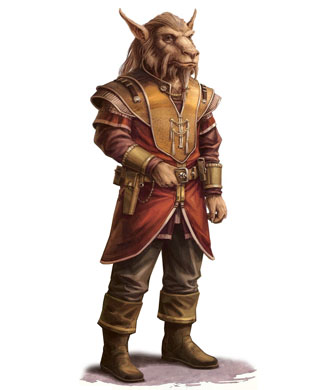
\includegraphics[width=1\linewidth]{../img/species/bothan}
\end{minipage}
\hfill
\begin{minipage}{0.7\textwidth}\raggedleft
	\begin{itemize}
		\item \textbf{Seuil de blessure :} 10 + Vigueur 
		\item \textbf{Seuil de stress :} 11 + Volonté 
		\item \textbf{Expérience de départ :} 100 XP
		\item \textbf{Capacité spéciale :} les Bothans commencent le jeu avec 1 rang en \textbf{Système D}. Ils ne peuvent cependant pas dépasser le rang 2 dans cette compétence à la création de perso. Ils commencent également avec 1 rang de \textbf{Persuasion}.
	\end{itemize}
\end{minipage}

\section*{Droïdes}
\noindent\begin{minipage}{0.3\textwidth}
	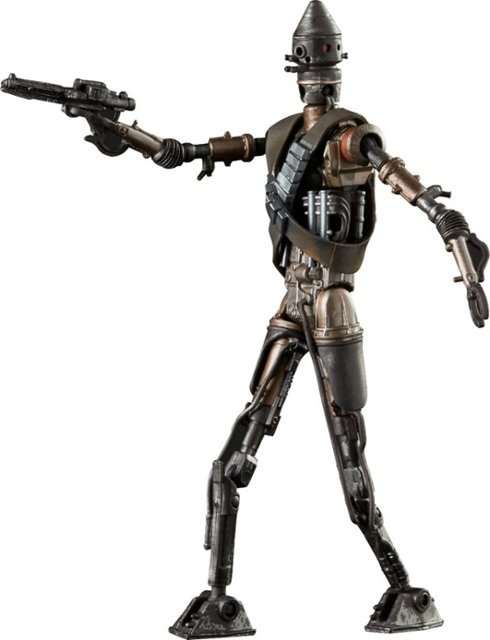
\includegraphics[width=1\linewidth]{../img/species/droid}
\end{minipage}
\hfill
\begin{minipage}{0.7\textwidth}\raggedleft
	\begin{itemize}
		\item \textbf{Seuil de blessure :} 10 + Vigueur 
		\item \textbf{Seuil de stress :} 10 + Volonté 
		\item \textbf{Expérience de départ :} 175 XP
		\item \textbf{Capacité spéciale :} les Droïdes ne mangent pas, ne dorment pas, ne respirent pas. La limitation d'implant est de 6. Une fois sa carrière choisie il gagne un rang dans 6 des 8 compétences de carrière (au lieu de 4), une fois sa spécialité choisie il gagne un rang dans 3 des 4 compétences de spécialités (au lieu de 2). \textbf{Inorganique :} les Droïdes étant inorganiques, les cuves bacta, stimpacks et tests de médecine sont inopérants. Ils récupèrent en se reposant. Autrement on peut s'en occuper avec des tests de mécaniques, les trousses de mécaniques s'utilisent comme les stimpacks. Pour plus de détails voir page 220. \textbf{Être mécanique : }les Droïdes ne peuvent pas être affectés par les pouvoirs de la Force qui influencent l'esprit, et ne peuvent non plus avoir de valeur de Force.
	\end{itemize}
\end{minipage}

\end{document}
